\hypertarget{overview}{%
\section{Overview}\label{overview}}

\hypertarget{on-the-usage-of-optional-c-keywords}{%
\section{On the usage of optional C
keywords}\label{on-the-usage-of-optional-c-keywords}}

The following chapter explain some keywords from the C language, that
are not needed for the computation to succeed, but provide additional
information to readers of the code and/or the compiler. The chapter is
based on \cite{modernc}, if not mentioned otherwise.

\hypertarget{inline}{%
\subsection{inline}\label{inline}}

The keyword `inline' (ch. 15.1) allows for code to be modularized by
functions, but without the overhead of an additional function call.
`inlining' a function f means that the compiler can take it and replace
every call to that function with the function body itself. This avoids
allocating new stack space and copying relevant variables for f
every time f is called. Furthermore the instructions of f might be seen in
a new context, allowing for further optimizations like eliminating dead
branches or avoiding repeated computation of already known values. The
keyword is only a hint for the compiler to inline the function. The
compiler might decide against inlining it, because the internal
optimization-algorithms classified the function as unsuitable for
inlining, for example if f was too big to be inlined. \cite[ch. 16]{styleguide} recommends using the keyword only for functions that have
three lines of code or less, which was followed in the present
implementation.

\hypertarget{restrict}{%
\subsection{restrict}\label{restrict}}

The `restrict'-qualifier (ch. 15.2) can only be applied to pointers and
tells the compiler that the pointer attributed with restrict is the only
one accessing the object pointed towards. If the compiler knows the
object in question is not aliased (e.g. accessed through multiple
pointers) it can perform further optimizations. The usage of this
keyword in the present implementation is not solely intended for the
compiler, but also for readers of the code, since it gives information
about how the pointer is intended to be used and what restrictions it is
confined by, that may be implicit without the keyword but now are made
explicit. Verifying the correctness of the usage of `restrict' is upon
the programmer not the compiler. It is a `promise' of the programmer to
the compiler, that the object is not aliased, as the compiler will
perform no checks to validate the claim made by restrict.

\hypertarget{const}{%
\subsection{const}\label{const}}

The following sub-chapter is based on \cite[ch. 1.4.2: Constants and Pointers]{cpointers}.

`const' is used in the present implementation to declare that the
pointer attributed with this keyword is pointing to a constant. This
means that the pointer can be used to read the values it points to, but
cannot modify them. It is mainly to clarify the intentions of the
programmer, for example if a function declaration contains a pointer to
a constant the function guarantees, that any data passed to this
function via the pointer to a constant will not be modified. This
guarantee is enforced at a compiler level. This is not to be confused
with a constant pointer or a constant pointer to a constant.

\hypertarget{functions---constant-generators}{%
\section{Functions - constant
generators}\label{functions---constant-generators}}

The following functions are from `AES\_encrypt\_generator.py' No
function in the following chapter does error checking, since they are
only intended for use inside a static, unchanging setting.

\hypertarget{galois-field-multiplication-lookup-table-generator}{%
\subsection{Galois field multiplication lookup table
generator}\label{galois-field-multiplication-lookup-table-generator}}

\hypertarget{description}{%
\subsubsection{Description}\label{description}}

As \cite{rijndael} recommends in chapter 4.1.1 Galois field multiplications
used in MixColumns were implemented as lookup tables in GFMLT. Since the
number of possible multiplication results is highly restricted in $GF(2^{8})$
the table storing all results uses neglibe memory. This avoids computing
the multiplications over and over. Furthermore in chapter 10.8.1 the
authors suggest, that implementing the multiplications as table lookups
makes the algorithm more resistant to timing attacks, since the finite
field multiplication performed in MixColumns is the only operation in
Rijdael that is not computed in constant time. In their 8-bit
implementation in chapter 4.1.1 they suggest only generating a table
where table t[a] = 02 * a, since multiplication with one is the factor
itself and multiplication with three can be efficiently archived by
XORing the result of the multiplication with two with the original
number: 03 * a = (02 * a) xor a 

To avoid leaking more timing data than
absolutely necessary the present implementation uses a lookup table for
all values, since this ensures that for each multiplication the CPU
(theoretically) does always the exact same amount of work, thus ensuring
it always takes the exact same amount of time. This size increase by 2 *
256b = 512 bytes (compared to the suggested implementation with only one
row) is negligible for our target of x86-CPU-systems, which today
typically feature memory sizes in the gigabyte range. 

\cite{rijndael} did not
make a mistake in their implementation suggestion though, since the
small lookup table variant was only suggested for memory constrained
8-bit environments. For 32-bit-architectures or wider they make even more
extensive use of lookup tables than the present implementation does
(compare ch. 4.2). This variant has not been used, since it reduces the
steps of the algorithm for each column in each round into four table
lookups accessing large tables crafted for this purpose, and four XOR
operations concatenating the lookup-results. This obscures the original
layout of the algorithm heavily and it was decided, that it should it to be recognizable
in the present implementation.

In the end the suggestions \cite{rijndael} makes regarding this topic have to
be taken with a grain of salt, since the extensive use of lookup tables
seems to enable new side channel attack vectors as previously discussed.

The lookup table used by the present implementation extends over two
dimensions: three rows for the multiplicators one, two and three and 256
columns to store the results of the multiplications with the numbers
denoting the column indices. Since the first dimension denotes the
multiplicator m, m - 1 accesses the right array for multiplication with
m, while the second dimension accesses the result for the value wanted.

\begin{quote}
The program needs to compute the multiplication of two times 114. This
means it has to access gal\_mult\_lookup[2-1]. For the result it
simply needs to use the second factor as the array index for the second
dimension. Thus the final array access to calculate 2 * 114 in $GF(2^{8})$ is
gal\_mult\_lookup[1][114]. For 3 * 86 it would be
gal\_mult\_lookup[2][86] etc.
\end{quote}

\hypertarget{implementation}{%
\subsubsection{Implementation}\label{implementation}}

\begin{lstlisting}
def mult_gal(a, b):
    """
    Multiplicates two numbers in the Galois Field specified by the AES-Standard.

    Algorithm specified under
    https://en.wikipedia.org/wiki/Finite_field_arithmetic#multiplication
    as a modiefied version of the "peasant's algorithm"
    Tested with https://www.ece.unb.ca/cgi-bin/tervo/calc2.pl
    """
    
    p = 0
    for i in range(8):
        if (a == 0) or (b == 0):
            break
        if b & 1:
            p ^= a
        b >>= 1
        a = ((a << 1)%256) ^ (-(a >> 7) & 0x1b)
    return p
\end{lstlisting}

This implementation of multiplication in $GF(2^{8})$ modulo $m(x) = x^8 + x^4 +
x^3 + x + 1$ is an adapted version from the `peasant's algorithm' as
described in
\cite{peasants}.
It takes two integers with values in range of 0-255 `a' and `b'. First
the variable `p' gets initialized with 0. The following loop gets
repeated at most eight times: If one of the two factors is 0 the
algorithm terminates. After that, `mult\_gal' evaluates, whether `b' is
odd by performing a bitwise AND-operation with `b' and 1. If the least
significant bit of `b' was toggled `p' gets XORed with `a' and the
result is stored in p. After that `b' gets bitshifted one to the right,
which equals division by two while ignoring the remainder. The last step
has two components. In the first component `a' gets shiftet by one to
the left, which equals multiplication by two. To ensure `a' remains
within the value-bounds of a byte (e.g. 0-255) the result is taken
modulo 256. The second component of the last step first shifts `a' to
the right by seven. This means that the most significant bit of `a' is
now its least significant bit, while all other bits are 0. By taking the
negative of this resulting value there are two possible outcomes: either
`a' before the shift had a 0 as its most significant digit, which after
its shift becomes its least significant one. Since all other digits are
also 0, the negative does not change anything: `a' contains (in base 2)
00000000. On the other hand if the most significant digit was a 1 before
the shift, the binary value of `a' after the shift would be 00000001 or
1. With the minus-sign this becomes -1 or (thanks to the two's
complement) 11111111. This is combined using the bitwise AND with 27.
The rationale behind this last component is simple: if `a' has the most
significant bit set to 1 prior to its shift to the right in the first
component, the bit goes out of scope for the byte value range, since it
is now the ninth bit, but a byte has only eight. In other words any
number with a ninth bit toggled in binary notation cannot belong to
$GF(2^{8})$. To stay within the range of 0-255 we have to perform modulo the
irreducible polynomial of the AES-Galois field, which is $m(x) = x^8 + x^4 +
x^3 + x + 1$ in polynomial representation (\cite[ch. 3.4.1]{rijndael},
100011011 in binary and 283 in base 10. Since this value is bigger than
a byte can hold it becomes 00011011 with the most significant digit cut
off, which is 1b in hexadecimal representation. If the most significant
bit of `a' was set prior to all of this, it has to be reduced modulo 1b
(which is represented by the bitwise XOR between the two components
here). The second component computes, whether the shifted `a' gets XORed
with 00000000 \& 1b (which is just 0) or 11111111 \& 1b (which is just
1b) depending on the value of 'a's most significant digit. The function
finishes by returning the value contained in p at the end of the loop.

\begin{lstlisting}
def gen_mult_lookup():
    """
    Generates a lookup table for the Galois-field-multiplication
    necessary in AES.
    """
    mult1 = bytearray(256)
    mult2 = bytearray(256)
    mult3 = bytearray(256)

    for i in range(256):
        mult1[i] = i
        mult2[i] = mult_gal(i, 2)
        mult3[i] = mult_gal(i, 3)

    return mult1 + mult2 + mult3
\end{lstlisting}

`gen\_mult\_lookup' generates the GFMLT for multiplications with 1, 2,
and 3 in $GF(2^{8})$ modulo m(x). It creates three byte arrays. The following
loop, iterating through the numbers 1 to 255, places the current
iteration value in the first array, the iteration value times two in the
second and the iteration value times three in the third byte array. The
function then returns the concatenation of all three arrays.

\hypertarget{testing}{%
\subsubsection{Testing}\label{testing}}

The results (App.XXX) were spot-checked against
https://www.ece.unb.ca/cgi-bin/tervo/calc2.pl with P(x) = 100011011.

\hypertarget{s-box-generator}{%
\subsection{S-box generator}\label{s-box-generator}}

\hypertarget{description-1}{%
\subsubsection{Description}\label{description-1}}

The S-box generator is used to generate the S-box needed in the
SubBytes-function. \cite[ch 3.4.1]{rijndael} gives two design criteria: Non-linearity
and Algebraic complexity.

The values of the AES S-box are computed by taking the value of the byte
that needs to be substituted, finding its inverse in $GF(2^{8})$ with the
irreducible polynomial $m(x) = x^8 + x^4 + x^3 + x + 1$ and applying an
affine transformation to that inverse.

\begin{figure}
\centering
\includegraphics[scale = 0.4]{data/figures/affinetrans.png} 
\caption{The affine transformation used in the AES S-box depicted as a matrix multiplication.}
\end{figure}

\begin{figure}
\centering
\includegraphics[scale = 0.4]{data/figures/S-box.png} 
\caption{The AES S-box. All values are in hexadecimal.}
\end{figure}


The S-box contains a substitution for every value an unsigned byte is
able to contain. Fig. XXX shows the S-box filled with values (in
hexadecimal) the present implementation generates. To use it in this
table format one has to split the byte to substitute into its digits.
The most significant digit is used to look up the row, the least
significant shows the column in that row. The intersection shows the
substitution value.

\begin{quote}
The byte to substitute contains the hexadecimal value of b8. The most
significant digit is b, meaning the substitution value is located in the
b-row. The least significant digit is 8, meaning the substitution value
is located in the 8-column of the table. Therefore the substitution
value is 6c, because it is located, where the b-row and the 8-column
intersect each other.
\end{quote}

\hypertarget{implementation-1}{%
\subsubsection{Implementation}\label{implementation-1}}

\begin{lstlisting}
def mult_inv_gal():
    """
    Generates a table of the multiplicative inverse of the Elements
    contained within the AES-Galois-Field.

    It uses an unelegant brute-force-method.
    """
    list_start = [*range(1, 256)]
    list_res = [0]
    for i in range(256):
        for j in list_start:
            if mult_gal(i, j) == 1:
                list_res.append(j)
                list_start.remove(j)
    return bytearray(list_res)
\end{lstlisting}

This function generates the inverses for all values in $GF(2^{8})$. First it
generates a list with the values from 1 to 255. After that it creates
another list containing the element 0 (since 0 has no inverse). Now it
iterates through all 256 possible values p. For each p it goes through
`list\_start' and multiplies them in $GF(2^{8})$ modulo m(x) using the
previously mentioned `mult\_gal' function. Since multiplying a number x
with its inverse always results in the multiplicative identity 1, the
present implementation simply tries to multiply all elements in $GF(2^{8})$
with each other (basically a brute-force approach) to see if the product
equals 1. In that case the value r from `list\_start' is appended to
`list\_res' at the index of the current value of p. After that r is
removed from list\_start, since every p has only one inverse in $GF(2^{8})$
modulo m(x) (proven experimentally by multiplying all elements in $GF(2^{8})$
with each other and noting the occurrences of products equal 1). In the
end the function returns `list\_res' converted to a byte array,
containing numbers that are the inverses of the values of their indices
(eg. element in listindex 37 is the inverse to the number 37).

\begin{lstlisting}
def shift_left(byte, rot):
    """Implements a left bitwise circular shift for bytes."""
    temp = (byte << rot)%256
    byte = temp | ((byte >> (8-rot)))
    return byte
\end{lstlisting}

This function implements a left bitwise circular shift of a byte. It
takes two arguments, `byte' and `rot'. `byte' is an integer in the range
of 0-255 and rot is an integer, denoting the number of places `byte'
should be shifted by. It starts by applying a bitwise left shift to
`byte', shifting it `rot' times. The result is reduced by modulo 256,
since the result cannot leave the range denoted by an unsigned byte,
e.g. 0-255. The reduced result is placed into the variable `temp'. Now
the bits of `byte' that got shifted to the left and `cut off' by the
modulo operation have to be brought back to the right. For that we shift
`byte' 8 - `rot' bits to the right. Now the two `halves' get combined by
applying a bitwise OR to `temp' and the result of the rightshift. This
result is saved in `byte'. Finally the function returns `byte'.

\begin{lstlisting}
def gen_sbox():
    """Genereates the AES S-box"""
    mult_inv_table = mult_inv_gal()
    sbox = bytearray(256)
    j = 0
    for i in mult_inv_table:
        #affine transformation
        sbox[j] = i ^ shift_left(i, 1) ^ shift_left(i, 2) ^ shift_left(i, 3) ^ shift_left(i, 4) ^ 0x63
        j += 1
    return sbox
\end{lstlisting}

This function generates the S-box array. First it uses the
`mult\_inv\_gal' function to generate a list containing all
multiplicative inverse of the elements in $GF(2^{8})$. After that it
allocates a byte array with length 256 called `sbox' and initializes the
variable `j' with zero. Then it iterates through the array of inverses,
applying the affine transformation and storing the result in sbox. The
affine transformation is computed by XORing the list element with
versions of itself that have been shifted left via circular byteshift
one, two, three and four times. Finally the result gets XORed with 99 to
obtain the result of the transformation.
(https://en.wikipedia.org/wiki/Rijndael\_S-box\#forward\_s-box) The
function finishes by returning the S-box-byte-array.

\hypertarget{testing-1}{%
\subsubsection{Testing}\label{testing-1}}

Since this is a static function generating always the same array, the
resulting array was compared once with the table in \cite[Fig. 7](fips197)


\hypertarget{functions---encryption}{%
\section{Functions - encryption}\label{functions---encryption}}

The following functions are from `AES\_encrypt.c'
(`Implementation'-chapters) and `test\_AES\_encrypt.py'
(`Testing'-chapters). The following chapter is based on \cite{fips197} and the authors own
knowledge/opinions, if not mentioned otherwise.

\hypertarget{key-addition}{%
\subsection{Key Addition}\label{key-addition}}

\hypertarget{description-2}{%
\subsubsection{Description}\label{description-2}}

\begin{figure}
\centering
\includegraphics[scale = 0.4]{data/figures/addroundkey.png} 
\caption{Addition of the round key to to the state via bitwise XOR. a0,0 xor k0,0 = b0,0 etc.}
\end{figure}

In this transformation a round key is
combined with the state, thus modifying it. The combination is
accomplished using the bitwise XOR operation. The round key array is
derived from the initial cipher key using the key schedule. Containing
16 bytes, each round key is equally long to a block. Since there are N+1
round keys generated (where N is the number of rounds), each round uses
a different round key (5.1.4).

\hypertarget{implementation-2}{%
\subsubsection{Implementation}\label{implementation-2}}

\begin{lstlisting}
/*
 * Adds the roundkey to a block.
 */
inline void AddRoundKey(uint8_t * restrict bytes, 
                        const uint8_t * restrict keys)
{
        for(uint8_t i = 0; i < 16; i++) {
                bytes[i] ^= keys[i];
        }
}
\end{lstlisting}

This function is used to add the current round key to the current block.
It takes a restricted pointer to the first byte of the block the cipher
is currently operating on and a restricted pointer to a constant, which
points to the first byte of the round key, that is supposed to be used
currently. It proceeds to combine each of the sixteen bytes of the block
with a corresponding byte of the round key designated to the current
round using the bitwise XOR. The result is then stored in the block byte
used in the XOR operation, meaning that first byte one of the block will
be XORed with byte one of the round key and then the result will be
stored in place of byte one and so forth for all sixteen bytes.

Since the function is relativly short the `inline'-keyword is used to
save the overhead of an additional function call in tradeoff with a
bigger binary.

\hypertarget{testing-2}{%
\subsubsection{Testing}\label{testing-2}}

Since the function is fairly simple, it is not covered by the testing
suite.

\hypertarget{shift-rows}{%
\subsection{Shift rows}\label{shift-rows}}

\hypertarget{description-3}{%
\subsubsection{Description}\label{description-3}}

\begin{figure}
\centering
\includegraphics[scale = 0.4]{data/figures/shiftrows.png} 
\caption{The ShiftRows-transformation "rotates" the rows of the state (left) by different offsets, resulting in the state on the right}
\end{figure}

(rijndael)(p.37) states, that this transformation of the state represents a byte transposition, using
cyclical shifts with different offsets. The first row of the 4x4-Matrix
of 16 bytes that constitutes the so called state is not shifted at all,
the second row by one step to the left, the third row uses two steps and
the fourth row three.

According to (rijndael) this transformation step is needed to ensure
optimal diffusion of the state. The diffusion is supposed to protect
against differential and linear cryptanalysis. The authors further
elaborate the need for that in order to archive optimal diffusion all
offsets of the cyclical shifts have to be different.

Since there are multiple possibilities for different offsets and not all
of them provided equal protection studies of attacks against Rijndael
were analyzed. From the offsets that proved to be the most resistant the
simplest offset was chosen.

\hypertarget{implementation-3}{%
\subsubsection{Implementation}\label{implementation-3}}

\begin{lstlisting}
/*
 * Achieves the AES-ShiftRows by representing it as a series of array-assignments.
 */
void ShiftRows(uint8_t * restrict block, uint8_t * restrict tempblock)
{
        memcpy(tempblock, block, 16 * sizeof(uint8_t));

        block[1] = tempblock[5];
        block[2] = tempblock[10];
        block[3] = tempblock[15];
        block[5] = tempblock[9];
        block[6] = tempblock[14];
        block[7] = tempblock[3];
        block[9] = tempblock[13];
        block[10] = tempblock[2];
        block[11] = tempblock[7];
        block[13] = tempblock[1];
        block[14] = tempblock[6];
        block[15] = tempblock[11];
}
\end{lstlisting}

The function ShiftRows performs the ShiftRows-transformation on the
state. It takes a restricted pointer to the first byte of the block the
cipher is currently operating on and a restricted pointer to a temporary
block. First the content of the block is copied into the array the
tempblock-pointer is marking. After that the row shifts are represented
by assigning the bytes into their positions in the block after the
shifts from the tempblock, for example:

\begin{quote}
Since the eleventh byte of the original array (tempblock{[}10{]}) will
(after the rotations) always be in the third spot in the resulting array
(block{[}2{]}) we can simply assign the former to the latter. The first
byte (tempblock{[}0{]}) is mapped to itself and therefore is not
explicitly ``mentioned'' in the code, since an assignment to itself
would be redundant.
\end{quote}

The result, which is the ShiftRows-transformed state, can now be found
in the array marked with the block-pointer and used for further
transformations.

`temparray' is passed to the function as a pointer, because allocating
the array every time the function is called creates a conciderable
overhead.

\hypertarget{testing-3}{%
\subsubsection{Testing}\label{testing-3}}

\begin{lstlisting}
@pytest.mark.parametrize(
    ("input_block", "expected"),
    (
        ("63cab7040953d051cd60e0e7ba70e18c", "6353e08c0960e104cd70b751bacad0e7"),
        ("a761ca9b97be8b45d8ad1a611fc97369", "a7be1a6997ad739bd8c9ca451f618b61"),
        ("3b59cb73fcd90ee05774222dc067fb68", "3bd92268fc74fb735767cbe0c0590e2d")
    )
)
def test_ShiftRows(input_block, expected):
    """Tests the C-implementation of the ShiftRows-function"""
    ba = bytearray.fromhex(input_block)
    reference = bytearray.fromhex(expected)
    byte_array = ctypes.c_ubyte * len(ba)
    temp_array = ctypes.c_ubyte * len(ba)
    aeslib.ShiftRows(byte_array.from_buffer(ba), temp_array.from_buffer_copy(ba))
    assert ba == reference
\end{lstlisting}

The testfunction for ShiftRows possesses a decorator, which tells pytest
what parameters this function is supposed to be tested on. The function
itself accepts two variables, one for the input of the
ShiftRows-function labeled `input\_block' and a corresponding correct
output labeled `expected', which will be computed from the input, if the
ShiftRows-function behaves correctly. Values for both input variables
are expected to be strings of 16-byte hex numbers. Those numbers are
transformed into two seperate byte arrays, `ba' and `reference'. The
C-ShiftRows function accepts a pointer to an array of 16 unsigned bytes,
which contain the current state and a pointer to an array of 16 unsigned
bytes, which can be used as a temporary array. After the ShiftRows
function returns, the result of the transformation is contained in the
bytearray `ba'. `ba' is then compared to `reference'. pytest will mark
this test as passed, when all three comparisons of the transformed `ba'
and 'reference evaluated to true. The test vectors passed via the
decorator are from (fips197) and represent the expected transformations.

\hypertarget{mix-columns}{%
\subsection{Mix columns}\label{mix-columns}}

\hypertarget{description-4}{%
\subsubsection{Description}\label{description-4}}

The MixColumns-transformation is called a bricklayer permutation by
(rijndael), which operates on the state-matrix columnwise. The authors
mention multiple design criteria, they deemed important for this
particular transformation:

\begin{enumerate}
\def\labelenumi{\arabic{enumi}.}

\item
  \emph{The bricklayer transformation is supposed to operate on columns
  containing 4 bytes.} This aspect is supposed to aid with the optimal
  implementation of look-up tables on 32-bit architectures, thus
  ensuring a speedy computation of the transformation.
\item
  \emph{The operation should be linear over GF(2)}, meaning the Galois
  Field of the two elements 0 and 1. This property aides the authors in
  their so-called `Wide Trail Strategy' (p.126) which is supposed to
  protect against differential and linear cryptanalysis.
\item
  \emph{The diffusion achieved by this transformation is supposed to
  have ``relevant'' power.} The third property is again supposed to
  support the `Wide Tail Strategy'.
\item
  \emph{The authors put emphasis on the performance of this step on 8-bit
  CPUs.} They deemed this neccessary, as they feared that the MixColumns
  transformation would be ``the only step that good performance on 8-bit
  processors is not trivial to obtain for.''(p.39)
\end{enumerate}


\begin{figure}
\centering
\includegraphics[scale = 0.3]{data/figures/mixcolumn.png} 
\caption{The MixColumns-transformation, represented as matrix multiplication.}
\end{figure}

The transformation itself partitions the
state-matrix into four columns. Each of those columns is transformed
independently from the other three. A single column acts as a polynomial
over $GF(2^{8})$, which is multiplied modulo $x^4 + 1$ with a fixed polynomial. In
order to meet the aforementioned criteria regarding performance,
diffusion and to fullfill the additional condition of creating an
invertible transformation (in regards to encryption) the authors were
forced to impose conditions on the fixed polynomials (rijndael). For
example, performance was archived by using only simple values for the
coefficients of the fixed polynomial. The fixed polynomial c(x) Daemen
and Rijmen settled on is $c(x) = 03 * x^3 + 01 * x^2 + 01 * x + 02$. They
state, that since c(x) and the aforementioned modulo $x^4+1$ are coprime
the calculation is invertible. The matrix-multiplication, which is seen
in Fig XXXX, is a representation of the modular multiplication with a
fixed polynomial.

158 - 88 4.1.1. 

\hypertarget{implementation-4}{%
\subsubsection{Implementation}\label{implementation-4}}

\begin{lstlisting}
/*
 * Achieves the AES-MixColumns by representing each result byte as a series of
 * table-lookups XORed with each other.
 */
void MixColumns(uint8_t * restrict block, uint8_t * restrict tempblock, 
                const uint8_t (* restrict gal_mult_lookup)[256])
{
        memcpy(tempblock, block, 16 * sizeof(uint8_t));

        for(uint8_t i = 0; i < 16; i += 4) {

                block[i] = gal_mult_lookup[1][tempblock[i]] ^
                        gal_mult_lookup[2][tempblock[i+1]] ^
                        gal_mult_lookup[0][tempblock[i+2]] ^
                        gal_mult_lookup[0][tempblock[i+3]];

                block[i+1] = gal_mult_lookup[0][tempblock[i]] ^
                        gal_mult_lookup[1][tempblock[i+1]] ^
                        gal_mult_lookup[2][tempblock[i+2]] ^
                        gal_mult_lookup[0][tempblock[i+3]];

                block[i+2] = gal_mult_lookup[0][tempblock[i]] ^
                        gal_mult_lookup[0][tempblock[i+1]] ^
                        gal_mult_lookup[1][tempblock[i+2]] ^
                        gal_mult_lookup[2][tempblock[i+3]];

                block[i+3] = gal_mult_lookup[2][tempblock[i]] ^
                        gal_mult_lookup[0][tempblock[i+1]] ^
                        gal_mult_lookup[0][tempblock[i+2]] ^
                        gal_mult_lookup[1][tempblock[i+3]];
        }
}
\end{lstlisting}

The function MixColumns takes multiple arguments. First it takes a
restricted pointer to the first byte of the block the cipher is
currently operating on, followed by a restricted pointer to a temporary
block and lastly the function gets a restricted pointer to the constant,
multi-dimensional GFMLT. MixColumns starts by copying the current state
from `block' into `tempblock'. After that it iterates through every row
by processing 4 consecutive bytes at a time, before it moves to the
following for consecutive bytes of `block'. Each Byte in `block' becomes
the result of four Galois field multiplications combined through the
bitwise XOR-operation, which represents the Galois field addition. The
multiplications are implemented as lookups in the GFMLT and combine the
coefficients of the fixed polynomial c(x) with the bytes of the current
row. After processing all four rows and returning, MixColumns has
written the results of this transformation in place of the current block
being processed.

\hypertarget{testing-4}{%
\subsubsection{Testing}\label{testing-4}}

\begin{lstlisting}
<# Vectors from [FIPS 197] Appendix C, Rounds 1, 2, 3
@pytest.mark.parametrize(
    ("input_block", "expected"),
    (
        ("6353e08c0960e104cd70b751bacad0e7", "5f72641557f5bc92f7be3b291db9f91a"),
        ("a7be1a6997ad739bd8c9ca451f618b61", "ff87968431d86a51645151fa773ad009"),
        ("3bd92268fc74fb735767cbe0c0590e2d", "4c9c1e66f771f0762c3f868e534df256")
    )
)
def test_MixColumns(input_block, expected):
    """Tests the C-implementation of the MixColumns-function"""
    ba = bytearray.fromhex(input_block)
    reference = bytearray.fromhex(expected)
    byte_array = ctypes.c_ubyte * len(ba)
    temp_array = ctypes.c_ubyte * len(ba)
    gal_mult_lookup_array = ctypes.c_ubyte * len(gal_mult_lookup)
    aeslib.MixColumns(byte_array.from_buffer(ba), temp_array.from_buffer_copy(ba),
                      gal_mult_lookup_array.from_buffer(gal_mult_lookup))
    assert ba == reference
\end{lstlisting}

Like other testing functions the test vectors for pytest to review are
provided via decorator. They are copied from (fips197) to ensure
correctness. The function takes one argument which represents the state
before a MixColumns transformation and one argument, which represents
the state after said transformation. Both are expected to be strings
containing the bytes encoded in hexadecimal notation. `input\_block'
gets converted to the bytearray `ba' and is then passed along with
another temporary sixteen-byte-array on towards the C-implementation of
the MixColumns-function. After the latter function returns, ba contains
the result of the desired transformation. pytest now compares each
output state to the corresponding test vector value to determine if the
MixColumns-implementation works correctly.

\hypertarget{substitute-bytes}{%
\subsection{Substitute bytes}\label{substitute-bytes}}

\hypertarget{description-5}{%
\subsubsection{Description}\label{description-5}}

\begin{figure}
\centering
\includegraphics[scale = 0.4]{data/figures/subbytes.png}
\caption{SubBytes applies the S-box substitution to every byte of the
state}
\end{figure}

Being the only non linear transformation, SubBytes is labeled a
bricklayer permutation by (rijndael) that applies byte substitution to
each byte of the state. This substitution is facilitated throught the
AES Sbox, which was already discussed in more detail earlier. AES uses
only this one Sbox, although the authors mention, that Rijndael ``could
as easily be defined with different S-boxes for every byte.'' (p.35).
They descided against it, because one key criteria during the
developement process for them was simplicity (ch.~5.2). Rijmen and
Daemen argue, that simplicity is an important contributer towards a
correct implementation, that it helps to get more people to review it,
since it is easier than reviewing more complex software and that it may
aide the notion it is easier to attack, thus motivating more of such
attacks. They further elaborate that the latter two points contribute to
the cryptographic credebility of the algorithm, especially if out of
many tries no successful attack can be mounted. Furthermore simpicity as
a design criterion was used to balance the security with the factors
efficiency and versatility. This simplicity was partially archived by
designing the algorithm following the principle of what they call
``symmetry''. Their tenet of symmetry within the round transformation
(ch.~5.3.2) " implies that it treats all bits of the state in a similar
way." (p.66). They explain that this imposes some restrictions, amongst
others the requirement to use only one sbox for the whole state in their
non-linear step. Symmetry across all rounds (ch.~5.31.) dictates that
all rounds have to be identical. This keeps the specification and
implementation short, since only one round has to be described/expressed
in code. This tersness in definition is also of benefit for hardware
implementations, since there has to be only one circuit designed to
implement all rounds, instead of one circuit per round. This tersness
also has the consequence, that only one Sbox can be used for all rounds
(contrary to DES (XXX)).

\hypertarget{implementation-4}{%
\subsubsection{Implementation}\label{implementation-4}}

\begin{lstlisting}
/*
 * Substitutes all bytes in a block with bytes from a sbox.
 */
inline void SubBytes(uint8_t * restrict bytes, const uint8_t * restrict sbox)
{
        for(uint8_t i = 0; i < 16; i++) {
                bytes[i] = sbox[bytes[i]];
        }
    
}
\end{lstlisting}

The SubBytes-implementation is pretty straightforward. The function
recieves two restricted pointers, one called `bytes', pointing to the
first byte of the current state, and one pointer to a constant array,
which contains the sbox to be used. The function now iterates through
`bytes', assigning every element from that array a new value by
accessing the element of the `sbox'-array, which corresponds to the
value in the current `bytes' element.

\hypertarget{testing-5}{%
\subsubsection{Testing}\label{testing-5}}

Since the function is fairly simple, it is not covered by the testing
suite.

\hypertarget{full-block-encryption}{%
\subsection{Full block encryption}\label{full-block-encryption}}

\hypertarget{description-6}{%
\subsubsection{Description}\label{description-6}}

To encrypt one block of AES the whole cipher with all rounds has to be
executed. One round consists of four steps, which represent the four
transformation employed in the encryption algorithm. The order of those
transformations for each round r is:

\begin{enumerate}
\def\labelenumi{\arabic{enumi}.}

\item
  SubBytes
\item
  ShiftRows
\item
  MixColumns
\item
  AddRoundKey
\end{enumerate}

If N is the number of rounds specified by the encryption standard then
the algorithm will execute N-1 * r, while the Nth round omits the
MixColumns step, but is otherwise identical. Before the first round one
additional AddRoundKey is performed on the state.

\hypertarget{implementation-5}{%
\subsubsection{Implementation}\label{implementation-5}}

\begin{lstlisting}
void encryptBlock(uint8_t * restrict block, uint8_t * restrict tempblock, 
                  const uint8_t * restrict keys, const uint8_t rounds, 
                  const uint8_t * restrict sbox, 
                  const uint8_t (* restrict gal_mult_lookup)[256])
{   
        uint8_t ikeys = 0;
        AddRoundKey(block, keys);
        ikeys += 16;

        for(uint8_t i = 0; i < rounds - 1; i++) {   
                SubBytes(block, sbox);
                ShiftRows(block, tempblock);
                MixColumns(block, tempblock, gal_mult_lookup);
                AddRoundKey(block, &keys[ikeys]);
                ikeys += 16;
        }
        
        SubBytes(block, sbox);
        ShiftRows(block, tempblock);
        AddRoundKey(block, &keys[ikeys]);
}
\end{lstlisting}

The present implementation of the Cipher takes multiple arguments. Like
in all other functions a restricted pointer to the first element in the
state array is provided. The second argument is a restricted pointer to
another bytearray of length sixteen, that can be used to store temporary
values. The third argument is a restricted pointer to a constant
bytearray, which contains the roundkeys. The next argument is a constant
byte denoting the number of rounds for the algorithm. It is passed to
provide future extensebility in case different key lengths are used and
thus different round numbers are needed, since this number depends on
the key length. The fifth argument is a restricted pointer to a constant
array containing the S-box values. The last argument is a restricted
pointer to a constant, multidimensional array containing the GLFMLT.

The function begins by allocation an unsigned byte on the stack and
assigning it the value of zero. This variable keeps track of the first
byte of the next key that is to be used in the function AddRoundKey,
thus has to be incremented by 16 after every call to the
AddRoundKey-function. The name is derived from ``\textbf{i}ndex of the
round\textbf{keys}''. Next the AddRoundKey-function is called with the
pointer to the current state and a pointer to the first round-key, which
is followed by the first increase of the `ikeys'-variable. Now the
rounds are executed in a for-loop, that counts from zero to the number
of rounds minus one. Every round consists of the following steps:
SubBytes is called with a pointer to the current state and a pointer to
the sbox, followed by a call of ShiftRows with a pointer to the current
state and the tempblock, then a call of MixColumns with pointers to the
current state, the temporary block and the GFMLT. Now comes a call to
AddRoundKey with a pointer to the current state and the memory address
`keys' would point towards, if it was increased by the amount stored in
`ikeys'. The latter passes on the starting address of the bytearray of
the next round key to be used by AddRoundKey. The last part of each
round is the increase of the `ikeys'-counter. After exiting the loop the
function executes one more round without the call to MixColumns and the
increase of the `ikeys'-counter variable and then it returns.

\hypertarget{testing-6}{%
\subsubsection{Testing}\label{testing-6}}

\begin{lstlisting}
@pytest.mark.parametrize(
    ("plaintext", "key", "expected"),
    (
        (
            "3243f6a8885a308d313198a2e0370734",
            "2b7e151628aed2a6abf7158809cf4f3c",
            "3925841d02dc09fbdc118597196a0b32"
        ),
    )
)
def test_EncryptBlock(plaintext, key, expected):
    """Tests the C-implementation of the AES-Encryption of a single block"""
    ba = bytearray.fromhex(plaintext)
    byte_array_block = ctypes.c_ubyte * len(ba)

    reference = bytearray.fromhex(expected)
    baKey = expand_key(key)
    byte_array_key = ctypes.c_ubyte * len(baKey)

    temp_array = ctypes.c_ubyte * len(ba)
    sbox_array = ctypes.c_ubyte * len(sbox)
    gal_mult_lookup_array = ctypes.c_ubyte * len(gal_mult_lookup)
    

    aeslib.encryptBlock(byte_array_block.from_buffer(ba), temp_array.from_buffer_copy(ba),
                        byte_array_key.from_buffer(baKey), 10, sbox_array.from_buffer(sbox),
                        gal_mult_lookup_array.from_buffer(gal_mult_lookup))
    assert ba == reference
\end{lstlisting}

Our first function to test the correctness of our cipher is marked with
a pytest-decorator, that contains a testvector from (fips197). The
function itself takes three arguments, one called `plaintext', one
called `key' and one called `expected'. All three are supposed to
contain a hexadecimal representation of bytesequences in a string
format. The function starts by converting `plaintext' and `expected into
bytearrays. It then generates the round keys from 'key' by calling the
function expand\_key. The `encryptBlock' function now recieves all
neccessary arguments via the ctypes-interface, namely the
plaintext-bytearray, a temporary array, the bytearray containing the
expanded keys, the number of rounds, the S-box array generated with one
of the generator functions and the GLFMLT array, which has been
generated before like the S-box. pytest marks this test as passed, when
the encrypted bytearray matches the bytearray generated from the
`expected'-value of the testvector.

\begin{lstlisting}
def test_EncryptBlockRandom():
    """
    Tests the C-implementation of the AES-Encryption of an arbitrary number of individual blocks.
    Plaintext and Key are randomized each time.
    """
    ba = bytearray(16)
    byte_array_block = ctypes.c_ubyte * len(ba)
    key = bytearray(16)
    baKey = bytearray(176)
    byte_array_key = ctypes.c_ubyte * len(baKey)
    temp_array = ctypes.c_ubyte * len(ba)
    sbox_array = ctypes.c_ubyte * len(sbox)
    gal_mult_lookup_array = ctypes.c_ubyte * len(gal_mult_lookup)
    for i in range(100): #arbitrary number of rounds
        key = urandom(16)
        baKey = expand_key(key.hex())
        b = urandom(16)
        ba = bytearray(b)
        aes_reference = pyaes.AESModeOfOperationECB(key)
        reference = aes_reference.encrypt(b)
        aeslib.encryptBlock(byte_array_block.from_buffer(ba), temp_array.from_buffer_copy(ba),
                        byte_array_key.from_buffer(baKey), 10, sbox_array.from_buffer(sbox),
                        gal_mult_lookup_array.from_buffer(gal_mult_lookup))
        assert ba == reference
\end{lstlisting}

The second test generates an arbitrary amount of random plaintexts and
keys (in the present version of the implementation 100 of each) and
compares them against a reference implementation of AES, in our case the
`pyaes'-library (XXX). The first part is nearly identical to the
previous test function. After setting up all the byte arrays the
function enters a loop though. For every iteration Python fills the
key-bytearray and the plaintext-bytearray with 16 random bytes each. It
uses the urandom-function from the os library (XXX) to generate those
random bytes. The byte-sequences are now processed independently by the
pyaes implementation (in electronic codebook mode) and the present
implementation. This function is marked as passed, when the encryptions
initialized with random plaintexts and key pass for every iteration. To
create a more throrough version of the test one can increase the number
of iterations at expense of decreased performance. This test is used in
addition to the normal test, because it ensures the implementation and
all of its components (for example SubBytes) can not only handle the
testvector, but all possible values that fulfill the requirements.

\hypertarget{encryption-of-multiple-consecutive-blocks}{%
\subsection{Encryption of multiple consecutive
blocks}\label{encryption-of-multiple-consecutive-blocks}}

\hypertarget{description-7}{%
\subsubsection{Description}\label{description-7}}

Although not explicitly required in context of this work, the present
implementation contains the possibility to encrypt multiple consecutive
blocks. With that it enables encryption of for example messages larger
than sixteen bytes or even files. 

(paar) (ch.~5.1.1) describes
encryption schemes like found in the present implementation the simplest
block cipher modes of operation, called `Electronic Codebook Mode'.
Every cipher block is generated by simply encrypting the plaintext with
the round keys and appending the encrypted blocks. The first advantage
of this method is that no synchronization between the en- and decrypting
party is necessary, since each block can be processed independently of
each other. Bit errors do not propagate through the whole ciphertext but
are confined to the block they occured in. The implementation has also
the potential to become very fast, thanks to the posibility of
processing different blocks on different cores, thus enabling
parallelisation of en- and decryption. 

The weaknesses of this mode
should not be underestimated though. Due to the fact that every block is
encrypted with the same key, the same plaintexts will generate the same
outputs. If the ciphertext is examined at a block level this is not of
greater significance, since AES guarantees that each encrypted block is
indistinguishable from randomly generated bytes. But if the plaintext as
a whole gets analyzed patterns may emerge. Those patterns leak
information about what parts of the plaintext contain the same 128-bit
sequence, because those parts also share a (different) bit seqence in
the corresponding ciphertext. Furthermore, a third party watching an
exchange encrypted in `Electronic Codebook Mode' can tell, when the same
message is send twice, or if the header of different messages is the
same, for examle if each message was using the same salutation. (paar)
demonstrates two attack avenues, that are a direct result of ECB. The
first one exploits the ECB-encrypted communication channel between two
banks. Here the attacker A just needs to open one account on both banks
and review the communication channel for patterns from test transactions
he is sending between the two accounts. If the banks do not rotate keys
A will soon know which encrypted blocks belong to his account number and
which block denote the recieving account. After learning that they can
exchange all blocks they know as reserved for the number of the
recieving account with the blocks for their own account number and
divert all transactions between the two banks to A's account.

\begin{figure}
\centering
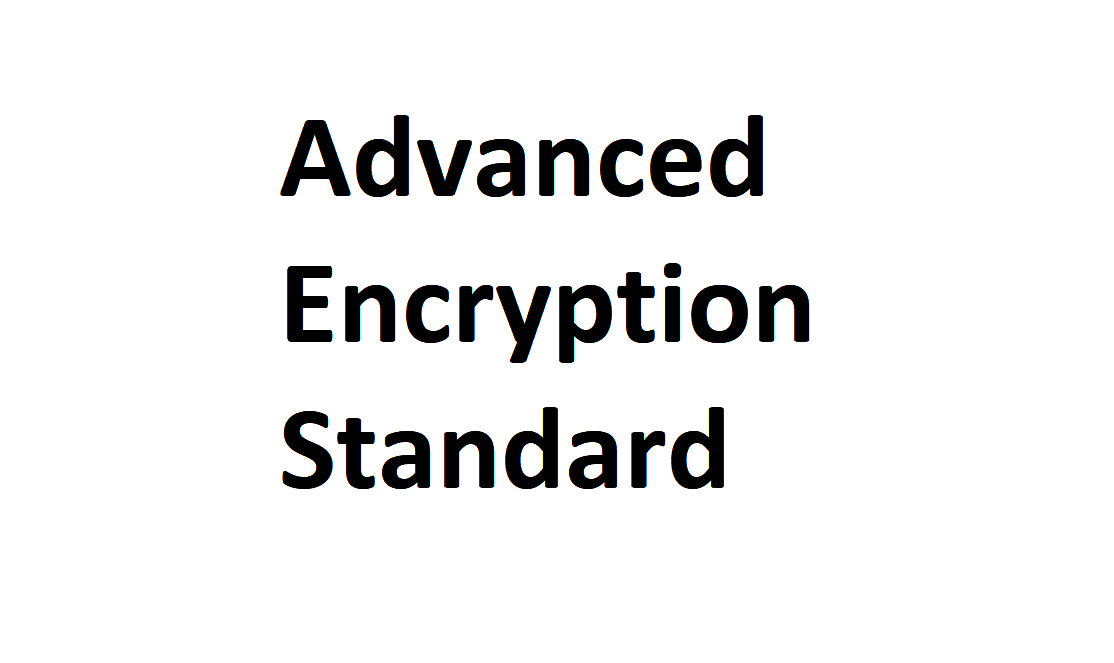
\includegraphics[scale = 0.4]{data/figures/aes.png} 
\caption{The unencrypted bitmap-file converted to a .png-file.}
\end{figure}

\begin{figure}
\centering
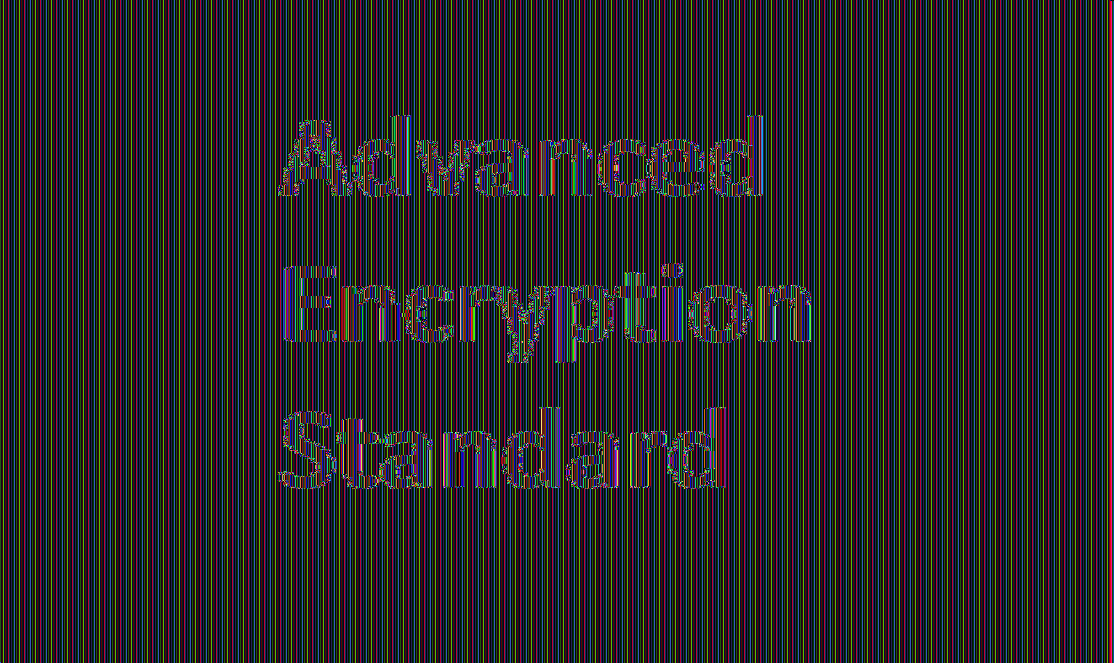
\includegraphics[scale = 0.4]{data/figures/aesECB.png} 
\caption{The bitmap-file encrypted with AES in ECB mode and converted to a .png-file. The writing "Advanced Encryption Standard" is clearly readable, despite the encryption.}
\end{figure}

\begin{figure}
\centering

\includegraphics[scale = 0.4]{data/figures/aesCTR.png} 
\caption{The bitmap-file, encrypted with AES in CTR mode and converted to a .png-file. To the naked eye the content of the picture is indistinguishable from noise.}
\end{figure}

The other
attack avenue is the emergence of patterns visible to the naked eye. For
this example we created an image in the bitmap format(Fig. XXX). This
image was encrypted with a modified variant of the present
implementations file encryption mode. The modification (inserted just
before the while-loop) ensures that the header of the .bmp-file is
preserved and not corrupted by the encryption. It reads the first 55
bytes (since the header is 54 bytes long
(https://www.daubnet.com/en/file-format-bmp)) and writes them to the
encrypted file without encrypting them. After that, the rest of Fig. XXX
is read, encrypted and appended. The result Fig. XXX, albeit encrypted
with an algorithm concidered secure, shows a clear and readable pattern.
For comparison we used the `pyaes'-library to encrypt the image in the
same way with the same key and preservation method of the header, but
applied the Counter Mode of Operation. The result, displayed in Fig.
XXX, demonstrates, that any visible pattern resulting from
ECB-encryption disappears with the right Block Cipher Mode of Operation.
(paar)(ch.5.1.5) describes how the Counter Mode is an example of block
cipher modes of operation that avoids such patterns. First an
initialization vector IV gets choosen. This ensures that every
encryption pass is as unique as the IV. Due to this fact it is
recommended to never reuse the IV. This IV is then concatenated counter.
This combination with the length of 128 bits is then encrypted with AES
and the password. The result is XORed with 128 bits of plaintext to
create the ciphertext. The counter is increased for each concecutive
block that needs to be encrypted. This way each block of plaintext is
XORed with an uniqe combiation of IV, nonce and key. This makes it
highly unlikely for two identical blocks of plaintext to be encrypted
into two identical blocks of ciphertext, thus avoiding leakage of
information.

The present implementation is required to use ECB, since it has to be
able to reproduce the testvectors from (fips197). Due to timeconstrains
it was decided not to implement two different block cipher modes of
operation.

\begin{figure}
\centering
\includegraphics[scale = 0.3]{data/figures/ECB_encryption.png}
\caption{ECB: Every block of plaintext is simply encrypted with a key.}
\end{figure}

\begin{figure}
\centering
\includegraphics[scale = 0.3]{data/figures/CTR_encryption.png}
\caption{CTR: Every block of plaintext is XORed with a combination of initialization vector (here: Nonce) and counter, encrypted by the key to form the ciphertext.}
\end{figure}


key = passwort, iterations = 20, salt = aeskurs
https://en.wikipedia.org/wiki/File:ECB\_encryption.svg
https://en.wikipedia.org/wiki/File:CTR\_encryption\_2.svg

In order for Electronic Codebook Mode to work correctly the bye array
containing the plaintext has to be padded though, as only byte arrays
with length l can be processed where l modulo 16 equals 0. Padding can
be implemented in multiple ways, this implementation does it as follows:

\begin{lstlisting}
def pad_input(ba):
    """pads bytearray to have a length % 16 = 0"""
    topad = 16 - len(ba) % 16
    if topad == 0:
        topad = 16 #ensures that last byte is always padding
    padding = bytearray([topad] * topad) # PKCS 5, 7
    return ba + padding
\end{lstlisting}

First it decides how many bytes the passed array is missing until the
length l of the array fulfills the requirement l modulo 16 equals 0. The
number of missing elements m is then appended m times to the array in
need of padding. If no padding is required a whole block gets padded.
This ensures the last byte of the decrypted string always contains the
information on how many bytes are padded and need to be removed, since
without this procedure a value for the last byte of one would be
ambiguous: does the last byte need to be removed since it is padding of
one or is it part of the message? This follows the concept of (PKCS \#7
RFC2315).

\begin{quote}
The array containing the plaintext is 357 bytes long. Since 357 modulo 16 = 5,
five bytes need to be added to the plaintext array. The present
implementation then adds an array containing the values \{5, 5, 5, 5,
5\} to the array.
\end{quote}

\hypertarget{implementation-6}{%
\subsubsection{Implementation}\label{implementation-6}}

\begin{lstlisting}
/*
 * Initializes the constant tables sbox, galois-field-multiplication-lookup and keys.
 * Performs AES-encryption on multiple, consecutive blocks.
 */
void encryptAES(uint8_t * restrict bytes, uint8_t * restrict initval, 
                   const size_t bytecount, const uint8_t rounds)
{   
        uint8_t sbox[256];
        uint8_t gal_mult_lookup[3][256];
        for(size_t i = 0; i < 256; i++) {
                sbox[i] = *initval++;
        }
        for(size_t i = 0; i < 3; i++) {
                for(size_t j = 0; j < 256; j++) {
                gal_mult_lookup[i][j] = *initval++;
                }
        }
        
        const uint8_t *keys = initval;
        uint8_t tempblock[16];
        
        for(size_t i = 0; i < bytecount; i += 16) {
                encryptBlock(&bytes[i], tempblock, keys, 
                             rounds, sbox, gal_mult_lookup);
        }
}
\end{lstlisting}

The function takes four arguments. The first one is a restricted pointer
to an array containing the bytes that need to be encrypted. The second
argument is a restricted pointer to an array containing the
initialization values: first the elements of the S-box, followed by the
bytes of the GFMLT, while the rest are the bytes of the round keys. The
third is a constant unsigned variable which width equals the wordwidth
of the CPU architecture the source code gets compiled on. The last
argument is a constant byte containing the number of rounds. The
function starts by allocation an array of 256 unsigned bytes called
`sbox'. After that another array named `gal\_mult\_lookup' is allocated,
but this time it is two-dimensional, using three times 256 unsigned
bytes. The name is derived from `\textbf{Gal}ois field
\textbf{mult}iplication \textbf{lookup}table'. Both are initalized with
the three following for-loops. The first loop reads the first 256 bytes
from `initvar' and assigns them to `sbox'. The following two nested
for-loops iterate through the two dimensions of `gal\_mult\_lookup' and
assign the results of the Galois field multiplications in $GF(2^{8})$ to the
respective dimensions of the array.

After populating the arrays the pointer has moved far enough through
`initvals' that it now points to the first byte of the first round key.
To make this more clear and to enable possible compiler optimizations we
create a new pointer named `keys' poining to a constant array, which is
in this case `initvals'. All future accesses to this array will be
throught `keys' or descendants of this pointer. The last step before
starting the encryption routine is the creation of an array of sixteen
unsigned bytes called `tempblock'. The next for loop starts the
encryption. Every iteration processes one block and increments the loop
index variable by sixteen, so that it can point to the next block to be
processed. In every iteration of this loop the function `enrcryptBlock'
is called with the address of the current block to encrypt, a pointer to
the temporary block, a pointer to the array containing the round keys, a
variable containing the number of rounds, a pointer to the sbox and a
pointer to the GFMLT.

Since parallelisation of the de- and encryption routine seems to be a
worthwhile endeavour for the future, this function was already designed
with that in mind. An allocation of the temporary block as a local
variable instead of a global one avoids the need for thread
synchronization, since every thread would use their own temporary block,
if every thread spawned would use this function as a starting point.

\hypertarget{testing-6}{%
\subsubsection{Testing}\label{testing-6}}

\begin{lstlisting}
def test_encrypt_aes():
    """Tests the C-implementation of the AES-Encryption on multiple, consecutive, random Blocks.
    """
    no_bytes = 2**15 #arbitrary number of bytes (has to be divisible by 16)
    ba = bytearray(no_bytes)
    byte_array_block = ctypes.c_ubyte * len(ba)
    key = bytearray(16)
    baKey = bytearray(176)
    initvals = bytearray(len(sbox) + len(gal_mult_lookup) + len(baKey))
    byte_array_initvals = ctypes.c_ubyte * len(initvals)
    for i in range(20): #arbitrary number of rounds
        key = urandom(16)
        baKey = expand_key(key.hex())
        initvals = sbox + gal_mult_lookup + baKey
        b = urandom(no_bytes)
        ba = bytearray(b)
        aes_reference = pyaes.AESModeOfOperationECB(key)
        aeslib.encryptAES(byte_array_block.from_buffer(ba),
                        byte_array_initvals.from_buffer(initvals), len(ba), 10)

        i = 0
        while (i < no_bytes):
            current_reference = aes_reference.encrypt(b[i:i+16])
            current_ba = ba[i:i+16]
            assert current_ba == current_reference

            i += 16
\end{lstlisting}

This testfunction is similar to the previously discussed
`test\_EncryptBlockRandom'. The major difference is that this function
is not resticted to testing sixteen bytes at a time. by adjusting
`no\_bytes' one can test as many consecutive blocks as memory and
patience permit. The for-loop again allows for automatic repetition of
this test to ensure the tested function can handle all byte permutation
within the specified range. Since the `pyaes'-library does not allow for
encryption of multiple consecutive blocks, a while-loop had to be added
in the end, that allows this external library to encrypt one block at a
time and compare it afterwards to the results of the present
implementation, which encrypts all blocks in one go. The test only
passes, if every block encrypted by the present implementation matches
the ciphertext produced by the `pyaes'-library. It ensures that longer
texts or files get encrypted correctly, as long as the passed parameters
are within the specified range.

\begin{center}\rule{0.5\linewidth}{0.5pt}\end{center}

\begin{itemize}

\item
  CPU central processing unit
\item
  GFMLT Galois-Field multiplication lookup table
\item
  $GF(2^{8})$ Galois field\ldots{}
\item
  ECB Electronic Codebook Mode
\end{itemize}

´
